\documentclass[11pt]{article}
\usepackage{amsmath}
\usepackage{tikz}
\usetikzlibrary{positioning, calc}
\usepackage[margin=1in]{geometry}
\usepackage{parskip}

\title{Block Diagram Reduction: Feedforward + Feedback}
\author{}
\date{}

\begin{document}
\maketitle

\section*{Block Diagram}

The feedforward-augmented feedback loop is shown below.  The reference $R(s)$
drives two paths simultaneously: the feedforward block $F(s)$ (direct) and the
error-forming junction (via feedback).

\begin{figure}[htbp]
\centering
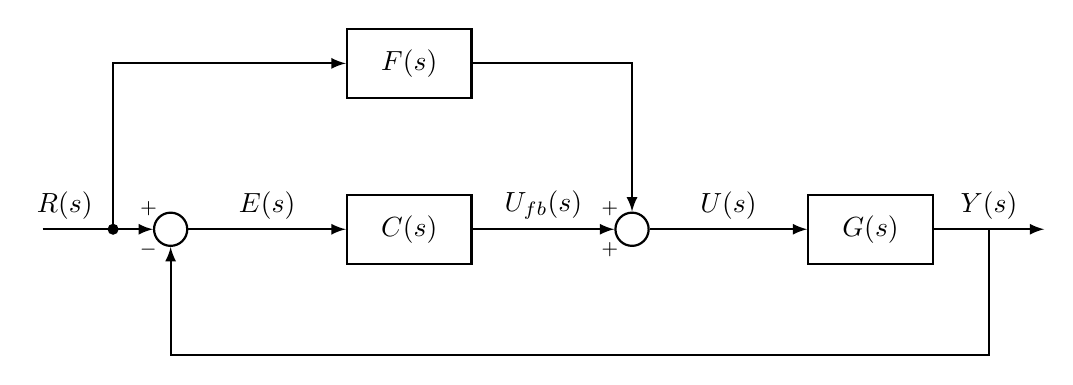
\begin{tikzpicture}[
  >=latex, thick,
  block/.style = {draw, rectangle, minimum height=2.5em, minimum width=4.5em},
  sum/.style   = {draw, circle, inner sep=0pt, minimum size=1.2em},
]
  \node[coordinate]                    (rin)   {};
  \node[sum,   right=1.4cm of rin]     (esum)  {};
  \node[block, right=2.0cm of esum]    (C)     {$C(s)$};
  \node[sum,   right=1.8cm of C]       (usum)  {};
  \node[block, right=2.0cm of usum]    (G)     {$G(s)$};
  \node[coordinate, right=1.4cm of G]  (yout)  {};

  \node[block, above=1.2cm of C]       (F)     {$F(s)$};

  \node[font=\scriptsize, inner sep=0pt, anchor=south east] at (esum.north west) {$+$};
  \node[font=\scriptsize, inner sep=0pt, anchor=north east] at (esum.south west) {$-$};
  \node[font=\scriptsize, inner sep=0pt, anchor=south east] at (usum.north west) {$+$};
  \node[font=\scriptsize, inner sep=0pt, anchor=north east] at (usum.south west) {$+$};

  \coordinate (rbranch) at ($(rin)!0.55!(esum)$);
  \draw[->] (rin)     -- node[above, pos=0.2]{$R(s)$}  (esum);
  \fill (rbranch) circle (2pt);

  \draw[->] (rbranch) |- (F);
  \draw[->] (F)       -| (usum);
  \draw[->] (esum)    -- node[above]{$E(s)$}  (C);
  \draw[->] (C)       -- node[above]{$U_{fb}(s)$} (usum);
  \draw[->] (usum)    -- node[above]{$U(s)$}  (G);
  \draw[->] (G)       -- node[above]{$Y(s)$}  (yout);

  \coordinate (fbk) at ($(G.east)!0.5!(yout)$);
  \draw[->] (fbk) -- ++(0,-1.6) -| (esum.south);
\end{tikzpicture}
\end{figure}

\section*{Node Equations}

Label each signal by inspecting every summing junction and block output:

\begin{align}
  E     &= R - Y                        \label{eq:error}      \\
  U_{fb}&= C\,E                         \label{eq:ufb}        \\
  U     &= U_{fb} + F\,R               \label{eq:usum}       \\
  Y     &= G\,U                         \label{eq:plant}
\end{align}

\section*{Algebraic Reduction}

Substitute \eqref{eq:error} into \eqref{eq:ufb}, then substitute both into
\eqref{eq:usum}:
\[
  U = C\bigl[R - Y\bigr] + F\,R.
\]

Substitute into \eqref{eq:plant}:
\[
  Y = G\Bigl\{C\bigl[R-Y\bigr] + F\,R\Bigr\}.
\]

Expand:
\[
  Y = GC\,R - GC\,Y + GF\,R.
\]

Collect all $Y$ terms on the left:
\[
  Y\bigl[1 + GC\bigr] = G\bigl[C + F\bigr]R.
\]

Divide both sides by $\bigl[1 + GC\bigr]$:

\[
  \boxed{T(s) = \frac{Y(s)}{R(s)} = \frac{G(s)\bigl[C(s)+F(s)\bigr]}{1+G(s)C(s)}}
\]

\section*{Interpretation}

The denominator $1 + G(s)C(s)$ is identical to the denominator of a pure
feedback loop.  Feedforward does not alter the characteristic equation and
therefore does not change the closed-loop poles.

The numerator $G(s)[C(s)+F(s)]$ shows that the effective forward-path gain is
the sum of the feedback controller and the feedforward controller.  When the
feedforward path is removed ($F(s)=0$), the expression reduces to the familiar
unity-feedback result:
\[
  T(s)\big|_{F=0} = \frac{G(s)C(s)}{1+G(s)C(s)}.
\]

\section*{Choosing $F$ for Zero Steady-State Error}

For a step reference, zero steady-state error requires $T(0) = 1$ (unity DC
gain).  Evaluating $T(s)$ at $s=0$:
\[
  T(0) = \frac{G(0)\bigl[C(0)+F(0)\bigr]}{1+G(0)C(0)} = 1.
\]

Solving for $F(0)$:
\begin{align*}
  G(0)\bigl[C(0)+F(0)\bigr] &= 1 + G(0)C(0) \\
  G(0)F(0)                  &= 1             \\
  F(0)                      &= \frac{1}{G(0)}.
\end{align*}

The DC gain of the feedforward block must equal the reciprocal of the plant's
DC gain.  Denoting the plant DC gain $K_{\mathrm{dc}} = G(0)$, the condition is simply
\[
  \boxed{F(0) = \frac{1}{K_{\mathrm{dc}}}.}
\]

The simplest controller that satisfies this is the constant gain $F(s) = 1/K_{\mathrm{dc}}$.
This is the \emph{proportional feedforward}: it scales the reference by the
inverse of the plant's steady-state gain, delivering exactly the input the
plant needs at steady state without waiting for error to accumulate.

Note that a feedback-only loop with an integrator ($C(s)$ containing $1/s$)
also achieves $T(0)=1$ by driving $C(0)\to\infty$.  Feedforward achieves the
same result without relying on infinite loop gain, which improves transient
response and allows smaller feedback gains.

\end{document}
